\chapter{Le courant électrique et ses effets}\label{ch:g8:electric-current-effects}

Le courant a marché, anonyme et utile, à travers cinq années de
circuits~: filaments allumés, \omterm{ex:g6:circuits-and-safety:motor}{moteurs} qui tournent, \omterm{ex:g6:circuits-and-safety:motor}{vibreurs} qui
sonnent. Cette année, l'électricité devient quantitative ---
appareils de mesure, \omterm{def:g6:measurement-in-science:measuring}{unités} et lois --- et nous ouvrons par un
inventaire~: que peut \emph{faire} un courant, exactement~? Trois
effets, en fin de compte, et tout le monde électrique est bâti avec
eux.

\section{Les trois effets}

\begin{proposition}[Les effets du courant
électrique]\label{prop:g8:electric-current-effects:three}
Un courant qui traverse la matière se manifeste par trois effets~:
\begin{enumerate}
  \item l'\emph{effet thermique}\index{effet thermique}~: tout
        courant échauffe le \omterm{def:g4:conductors-insulators:conductor}{conducteur} qu'il traverse ---
        doucement dans les bons fils, férocement dans les fils fins
        ou surchargés, jusqu'au blanc et à dessein dans les
        filaments et les grille-pain~;
  \item l'\emph{effet magnétique}\index{effet magnétique}~: un
        courant rend magnétiques ses environs --- un fil fait
        dévier l'aiguille d'une \omterm{def:g4:magnets-and-compass:compass}{boussole} voisine, et un fil enroulé
        devient un véritable \omterm{def:g1:magnets:magnet}{aimant}, avec des pôles, que l'on peut
        commander à volonté~;
  \item l'\emph{effet chimique}\index{effet chimique}~: en
        traversant certains \omterm{def:g3:solids-liquids-gases:liquid}{liquides}, un courant provoque des
        transformations chimiques --- il décompose l'eau en deux
        \omterm{def:g3:solids-liquids-gases:gas}{gaz}, argente des cuillères, charge et décharge toutes les
        \omterm{def:g3:first-electric-circuit:battery}{piles}.
\end{enumerate}
\end{proposition}

\begin{example}[L'effet thermique au travail]\label{ex:g8:electric-current-effects:heating}
Voulu~: les barreaux rougeoyants du grille-pain, la résistance
cachée de la bouilloire, le filament chauffé à blanc des vieilles
lampes, le \omterm{def:g7:short-circuits-safety:fuse}{fusible} construit pour \omterm{def:g2:ice-water-steam:meltfreeze}{fondre} le premier. Subi~: les
chargeurs de téléphone tièdes, le dessous brûlant des ordinateurs
portables --- et la menace du \omterm{def:g7:short-circuits-safety:device}{court-circuit}, que tu as étudiée comme
la signature du coupable. Un seul effet, serviteur et danger, dosé
par l'intensité avec laquelle le courant circule --- une dose que
nous apprendrons à \emph{\omterm{def:g6:measurement-in-science:measuring}{mesurer}} au chapitre suivant.
\end{example}

\begin{omfigure}
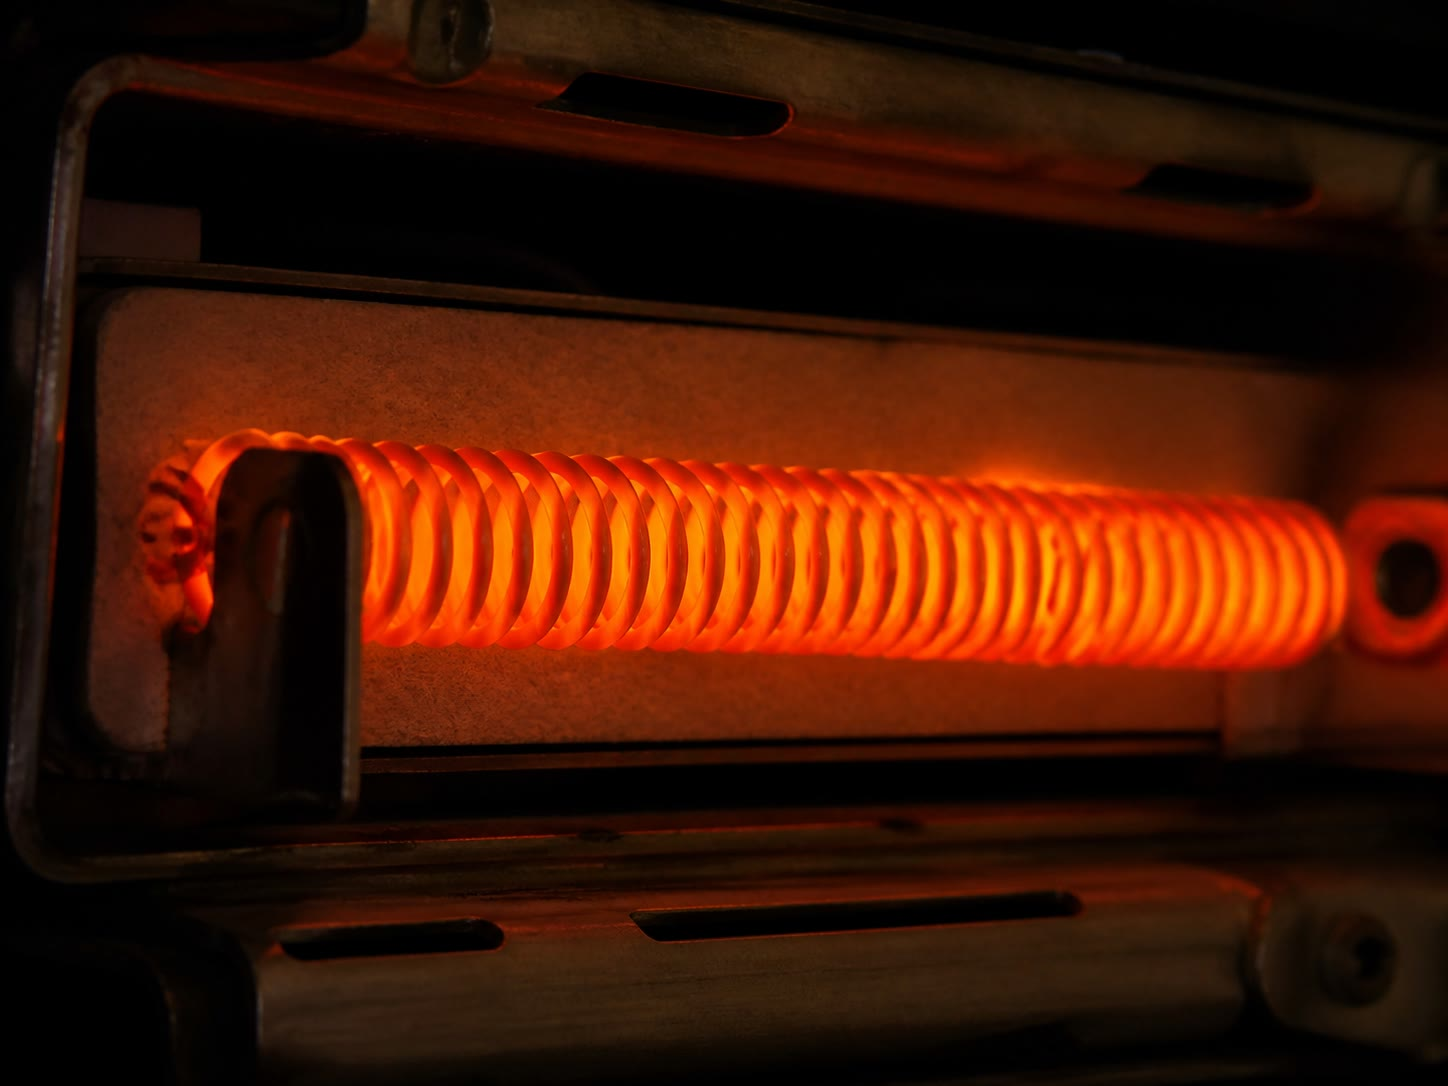
\includegraphics[width=0.5\linewidth]{images/book1/ai/g8-current-heating-coil.jpg}

{\small L'\omterm{prop:g8:electric-current-effects:three}{effet thermique}, incandescent~: le courant forcé dans la résistance du grille-pain la chauffe au rouge.}
\end{omfigure}

\section{Le courant fabrique des aimants}

\begin{example}[La boussole trahit le fil]\label{ex:g8:electric-current-effects:oersted}
Il y a deux siècles, pendant un cours, un physicien remarqua
qu'une aiguille de \omterm{def:g4:magnets-and-compass:compass}{boussole} tressaillait chaque fois qu'il fermait un
circuit sur la paillasse voisine. Ce tressaillement --- à peine un
frémissement d'aiguille --- fut le premier pont jamais vu entre
l'électricité et le magnétisme, deux sciences jusque-là aussi
séparées que la météo et la musique. Pose une \omterm{def:g4:magnets-and-compass:compass}{boussole} à côté d'un
fil et allume~: l'aiguille se déplace~; inverse le courant, et elle
se déplace dans l'autre sens. Le courant crée du magnétisme autour de
lui, avec un sens.
\end{example}

\begin{definition}[Électroaimant]\label{def:g8:electric-current-effects:electromagnet}
Un \emph{électroaimant}\index{électroaimant} est une bobine de fil
isolé --- souvent enroulée autour d'un noyau de fer --- qui devient
un \omterm{def:g1:magnets:magnet}{aimant} tant qu'un courant la traverse~: \omterm{def:g4:magnets-and-compass:poles}{pôle nord}, \omterm{def:g4:magnets-and-compass:poles}{pôle sud},
pouvoir d'\omterm{def:g1:magnets:magnet}{attirer} le fer, et tout le reste. Contrairement à tout
\omterm{def:g1:magnets:magnet}{aimant} de pierre, il obéit à un \omterm{ex:g3:first-electric-circuit:switch}{interrupteur}~: courant allumé, \omterm{def:g1:magnets:magnet}{aimant}
présent~; courant coupé, \omterm{def:g1:magnets:magnet}{aimant} disparu~; courant inversé, pôles
échangés.
\end{definition}

\begin{omfigure}
\begin{tikzpicture}[scale=0.85]
  \draw[thick, fill=omExo, fill opacity=0.3]
    (1.2,1.0) rectangle (5.4,1.9);
  \foreach \x in {1.5,2.1,...,5.1} {
    \draw[very thick, omDef] (\x,0.82) arc (200:340:0.35 and 0.5);
  }
  \draw[thick, omDef] (1.3,0.95) -- (0.4,0.4);
  \draw[thick, omDef] (5.3,0.95) -- (6.2,0.4);
  \node[below, font=\small] at (0.5,0.3) {vers la pile};
  \node[above, font=\small] at (3.3,2.05) {noyau de fer dans une bobine};
  \draw[thick] (7.4,1.05) ellipse (0.32 and 0.14);
  \draw[thick] (8.15,1.3) ellipse (0.32 and 0.14);
  \draw[thick] (7.5,1.6) ellipse (0.32 and 0.14);
  \node[right, font=\small] at (8.7,1.3)
    {trombones~: retenus tant que l'interrupteur est fermé};
\end{tikzpicture}

{\small L'\omterm{def:g8:electric-current-effects:electromagnet}{électroaimant}~: une bobine et un courant font un \omterm{def:g1:magnets:magnet}{aimant}
qu'un \omterm{ex:g3:first-electric-circuit:switch}{interrupteur} peut créer, détruire ou retourner.}
\end{omfigure}

\begin{example}[Le magnétisme commandable fait tourner le
monde]\label{ex:g8:electric-current-effects:uses}
La grue de la casse saisit une voiture avec un \omterm{def:g8:electric-current-effects:electromagnet}{électroaimant} et la
lâche en ouvrant un \omterm{ex:g3:first-electric-circuit:switch}{interrupteur} --- essaie donc avec un \omterm{def:g1:magnets:magnet}{aimant} de
pierre. Les serrures électriques, le claquement d'un relais, le
marteau de la sonnette (un \omterm{def:g8:electric-current-effects:electromagnet}{électroaimant} qui l'arrache vers le
timbre, coupe son propre courant et le laisse revenir en arrière~: le
grelot érigé en loi), la tête de lecture des vieux téléphones et,
surtout, tous les \omterm{ex:g6:circuits-and-safety:motor}{moteurs} électriques~: du magnétisme fabriqué par le
courant qui pousse contre des \omterm{def:g1:magnets:magnet}{aimants}, des milliers de fois par
seconde. L'\omterm{prop:g8:electric-current-effects:three}{effet magnétique} est le muscle de l'âge électrique.
\end{example}

\begin{method}[Bobiner un électroaimant]\label{met:g8:electric-current-effects:wind}
\begin{enumerate}
  \item enrouler un ou deux \omterm{def:g2:measuring-length:units}{mètres} de fil isolé fin en spires
        serrées et bien rangées autour d'un gros clou ou d'un
        boulon en fer, en laissant deux extrémités libres~;
  \item relier les extrémités à une \omterm{def:g3:first-electric-circuit:battery}{pile} par l'intermédiaire d'un
        \omterm{ex:g3:first-electric-circuit:switch}{interrupteur} (jamais directement pendant longtemps --- la
        bobine est presque un \omterm{def:g7:short-circuits-safety:device}{court-circuit} et s'échauffe~: l'\omterm{prop:g8:electric-current-effects:three}{effet
        thermique} chaperonne l'expérience)~;
  \item fermer brièvement l'\omterm{ex:g3:first-electric-circuit:switch}{interrupteur}~: la tête du clou attrape
        des trombones~; l'ouvrir~: ils tombent~;
  \item tester à la \omterm{def:g4:magnets-and-compass:compass}{boussole}~: les deux extrémités de la bobine se
        comportent comme un pôle N et un pôle S --- et s'échangent
        quand on retourne la \omterm{def:g3:first-electric-circuit:battery}{pile}.
\end{enumerate}
Plus de spires, prise plus ferme~: on dose le magnétisme en
bobinant.
\end{method}

\section{L'effet chimique}

\begin{example}[Du courant dans l'eau]\label{ex:g8:electric-current-effects:electrolysis}
Plonge deux mines de crayon reliées à une \omterm{def:g3:first-electric-circuit:battery}{pile} dans de l'eau rendue
légèrement conductrice (une cuillerée de cristaux de soude y aide),
et regarde~: de minuscules bulles filent des deux mines --- deux \omterm{def:g3:solids-liquids-gases:gas}{gaz}
différents, nés de l'eau elle-même, avec deux fois plus de \omterm{def:g6:mass-and-volume:volume}{volume} à
une mine qu'à l'autre. Le courant est en train de démonter l'eau en
ses deux composants invisibles. Cette porte entre l'électricité et la
chimie --- l'\emph{électrolyse} --- argente des cuillères bon marché,
arrache l'aluminium à son minerai, et appartient surtout à ton cours
de chimie~; la physique la salue et poursuit sa route.
\end{example}

\begin{example}[Toute pile est cet effet à
l'envers]\label{ex:g8:electric-current-effects:battery}
À l'intérieur de toute \omterm{def:g3:first-electric-circuit:battery}{pile}, c'est la chimie qui pousse le courant~:
une réserve d'\omterm{def:g5:everyday-energy:energy}{énergie} chimique met la marche en route et se dépense
en servant --- le vidage que tu connais depuis que la lampe de poche
a faibli. Les accumulateurs rechargeables bouclent la boucle~: le
chargeur \omterm{def:g2:pushes-and-pulls:force}{force} un courant \emph{à l'envers}, et l'\omterm{prop:g8:electric-current-effects:three}{effet chimique}
reconstruit la réserve. Du chimique à l'électrique, de l'électrique
au chimique~: un seul effet, deux sens, et toute l'industrie de la
\omterm{def:g3:first-electric-circuit:battery}{pile}.
\end{example}

\begin{remark}[Les effets comme détecteurs]\label{rem:g8:electric-current-effects:detect}
Les trois effets répondent à une question qui te laissait perplexe du
temps où tu étais l'apprenti au testeur~: comment \emph{voir} un
courant --- une marche invisible dans un fil \omterm{def:g7:light-sources-propagation:coats}{opaque}~? Par ses actes.
Un fil qui chauffe, une \omterm{def:g4:magnets-and-compass:compass}{boussole} qui tressaille, une bulle qui
file~: chacun trahit la marche. Tous les instruments de mesure du
courant jamais construits lisent l'un des trois effets --- et celui
qui attend au chapitre suivant lit le tressaillement magnétique,
raffiné en un cadran chiffré.
\end{remark}

\section{Exercices}

\begin{exercise}[$\star$]\label{exo:g8:electric-current-effects:1}
Nomme les trois effets du \omterm{def:g7:circuits-series-parallel:current}{courant électrique}, chacun avec un usage où
il nous sert.
\end{exercise}

\begin{exercise}[$\star$]\label{exo:g8:electric-current-effects:2}
Quel effet, dans chaque scène~: un \omterm{def:g7:short-circuits-safety:fuse}{fusible} qui fond~; \ une sonnette
qui martèle~; \ des bulles aux mines de crayon~; \ la lueur d'un
grille-pain~; \ la prise d'une grue de casse~?
\end{exercise}

\begin{exercise}[$\star$]\label{exo:g8:electric-current-effects:3}
Qu'a révélé le tressaillement de la \omterm{def:g4:magnets-and-compass:compass}{boussole} posée près de la
paillasse du cours~? Qu'arrive-t-il au tressaillement quand le
courant s'inverse~?
\end{exercise}

\begin{exercise}[$\star$]\label{exo:g8:electric-current-effects:4}
Cite trois pouvoirs qu'un \omterm{def:g8:electric-current-effects:electromagnet}{électroaimant} possède et qu'aucun \omterm{def:g1:magnets:magnet}{aimant} de
pierre ne peut égaler.
\end{exercise}

\begin{exercise}[$\star$]\label{exo:g8:electric-current-effects:5}
Dans la méthode de bobinage, pourquoi le fil doit-il être isolé~? Et
pourquoi la bobine ne doit-elle pas rester longtemps branchée sans
charge utile~?
\end{exercise}

\begin{exercise}[$\star$]\label{exo:g8:electric-current-effects:6}
Comment le grutier relâche-t-il la voiture~? Compare avec ce
qu'exigerait un \omterm{def:g1:magnets:magnet}{aimant} de pierre de \omterm{def:g2:pushes-and-pulls:force}{force} égale.
\end{exercise}

\begin{exercise}[$\star$]\label{exo:g8:electric-current-effects:7}
Quelle conversion d'\omterm{def:g5:everyday-energy:energy}{énergie} a lieu à l'intérieur d'une \omterm{def:g3:first-electric-circuit:battery}{pile} en
service~? Et à l'intérieur d'un accumulateur sur son chargeur~?
\end{exercise}

\begin{exercise}[$\star$]\label{exo:g8:electric-current-effects:8}
Pourquoi les trois effets sont-ils précieux comme
\emph{détecteurs}~? Quel effet l'instrument du chapitre suivant
raffinera-t-il en un nombre~?
\end{exercise}

\begin{exercise}[$\star\star$]\label{exo:g8:electric-current-effects:9}
La sonnette~: un \omterm{def:g8:electric-current-effects:electromagnet}{électroaimant} arrache le marteau vers le timbre,
mais le marteau en mouvement coupe son propre circuit~; un ressort le
ramène, ce qui rétablit le contact --- et ainsi de suite. Parcours un
cycle complet et explique pourquoi ce montage \emph{doit} grelotter
plutôt que tenir.
\end{exercise}

\begin{exercise}[$\star\star$]\label{exo:g8:electric-current-effects:10}
Un relais est un \omterm{ex:g3:first-electric-circuit:switch}{interrupteur} fermé par un \omterm{def:g8:electric-current-effects:electromagnet}{électroaimant}~: un petit
courant dans la bobine ferme des contacts qui portent un gros courant
dans un autre circuit. Explique pourquoi cela permet à un thermostat
délicat de commander sans danger un radiateur électrique vorace ---
et quels deux circuits ne se touchent jamais.
\end{exercise}

\begin{exercise}[$\star\star$]\label{exo:g8:electric-current-effects:11}
L'aiguille de ta \omterm{def:g4:magnets-and-compass:compass}{boussole} tressaille chaque fois qu'un fil caché dans
le mur porte du courant. Conçois à partir de ce fait un détecteur de
fils dans les murs~: protocole, ce que signifie un fort
tressaillement, et une limite honnête de l'instrument (pense à ce qui
fait bouger d'autre une aiguille de \omterm{def:g4:magnets-and-compass:compass}{boussole}).
\end{exercise}

\begin{exercise}[$\star\star\star$]\label{exo:g8:electric-current-effects:12}
Un \omterm{ex:g6:circuits-and-safety:motor}{moteur} électrique, en esquisse~: une bobine montée sur un \omterm{def:g6:sun-earth-moon:axisorbit}{axe} se
trouve entre les pôles d'un \omterm{def:g1:magnets:magnet}{aimant}~; le courant rend la bobine
magnétique~; les attractions et répulsions des pôles font tourner
l'\omterm{def:g6:sun-earth-moon:axisorbit}{axe} --- et, juste au moment où la bobine allait s'immobiliser
alignée, le courant qui la traverse est inversé, si bien qu'elle doit
poursuivre cet alignement pour toujours. Explique, pôle par pôle,
pourquoi cette inversion est indispensable --- que ferait le \omterm{ex:g6:circuits-and-safety:motor}{moteur}
sans elle~? (Tu viens d'expliquer pourquoi les \omterm{ex:g6:circuits-and-safety:motor}{moteurs} contiennent un
contact inverseur --- et la moitié de la façon dont l'âge électrique
fait tourner ses roues.)
\end{exercise}

\section{Problème~: l'atelier de l'inventeur}

\begin{problem}[{Problème du week-end --- une pile, trois effets,
cinq inventions~; une soirée dans l'atelier de
l'inventeur}]\label{pb:g8:electric-current-effects:1}
L'établi de l'atelier porte des \omterm{def:g3:first-electric-circuit:battery}{piles}, du fil, des clous en fer, une
\omterm{def:g4:magnets-and-compass:compass}{boussole}, deux mines de crayon, un bocal d'eau additionnée de
soude --- et un carnet d'inventions à moitié construites, à
évaluer.

\medskip\noindent\textbf{Partie I --- faire l'inventaire.}
\begin{enumerate}
  \item Esquisse le banc d'essai des trois effets de l'atelier~:
        pour une \omterm{def:g3:first-electric-circuit:battery}{pile} et un \omterm{ex:g3:first-electric-circuit:switch}{interrupteur}, décris un montage qui
        montre les trois effets à la fois (un fil fin qui chauffe,
        une \omterm{def:g4:magnets-and-compass:compass}{boussole} à côté d'un \omterm{def:g4:conductors-insulators:conductor}{conducteur}, le bocal dans la
        boucle). Dans quelle disposition les trois démonstrations
        doivent-elles se trouver --- \omterm{def:g4:series-circuits:series}{en série} ou \omterm{def:g5:series-parallel-circuits:parallel}{en dérivation} ---
        pour qu'un seul \omterm{ex:g3:first-electric-circuit:switch}{interrupteur} les commande toutes~?
  \item Le fil fin de démonstration s'échauffe alors que les gros
        fils d'alimentation restent froids, dans la même boucle.
        Quel fait du premier chapitre sur la boucle \omterm{def:g4:series-circuits:series}{en série} rend
        cela \emph{plus} intéressant qu'il n'y paraît --- qu'est-ce
        qui est égal dans les deux fils, et qu'est-ce qui diffère~?
  \item La \omterm{def:g4:magnets-and-compass:compass}{boussole} tressaille vers l'est quand l'\omterm{ex:g3:first-electric-circuit:switch}{interrupteur} se
        ferme. Quels deux changements, faits ensemble, laisseraient
        le tressaillement exactement tel qu'il était~?
  \item Les bulles filent deux fois plus vite d'une mine de crayon
        que de l'autre. Que cela suggère-t-il sur les deux
        composants de l'eau~? (La chimie confirmera le rapport.)
\end{enumerate}

\medskip\noindent\textbf{Partie II --- évaluer les inventions.}
\begin{enumerate}[resume]
  \item Invention~: «~la sonnette silencieuse~» --- un
        \omterm{def:g8:electric-current-effects:electromagnet}{électroaimant} qui tire une fois un marteau feutré et le
        maintient jusqu'au relâchement du bouton. Quelle pièce du
        mécanisme classique de la sonnette l'inventeur doit-il
        \emph{supprimer}, et qu'entendra le visiteur~?
  \item Invention~: «~le trieur magnétique~» --- de la ferraille
        sur un tapis roulant passe sous un \omterm{def:g8:electric-current-effects:electromagnet}{électroaimant} qui en
        extrait le fer et l'acier. Que se passe-t-il au bac de
        largage, et pourquoi le trieur laisse-t-il les canettes en
        aluminium sur le tapis (deux faits sur les \omterm{def:g1:magnets:magnet}{aimants}, vus les
        années précédentes, répondent)~?
  \item Invention~: «~le retourne-pôles~» --- une \omterm{def:g4:magnets-and-compass:compass}{boussole} montée
        au-dessus d'une bobine, qui bascule chaque fois qu'un
        \omterm{ex:g3:first-electric-circuit:switch}{interrupteur} caché retourne la \omterm{def:g3:first-electric-circuit:battery}{pile}. Quelle propriété du
        magnétisme fabriqué par le courant est exploitée~?
  \item Invention~: «~l'électrolyseur éternel~» --- un argentage
        alimenté par une \omterm{def:g3:first-electric-circuit:battery}{pile} qui «~se recharge elle-même grâce à
        l'argentage~». Oppose ton veto, en citant les deux sens de
        la \omterm{def:g3:first-electric-circuit:battery}{pile} du chapitre et une loi plus ancienne sur l'\omterm{def:g5:everyday-energy:energy}{énergie}.
\end{enumerate}

\medskip\noindent\textbf{Partie III --- le chef-d'œuvre de la
soirée.}
L'inventeur termine par un jeu de grue pour la fête foraine~: un
manche à balai, un petit \omterm{def:g8:electric-current-effects:electromagnet}{électroaimant} au bout de câbles, un bac de
babioles en fer.
\begin{enumerate}[resume]
  \item Écris le scénario du coup gagnant en langage d'effets~: que
        se passe-t-il à la «~prise~», pendant le déplacement, et au
        «~lâcher~»~?
  \item Les visiteurs se plaignent que la grue laisse tomber les
        lots en plein déplacement dès que la vieille \omterm{def:g3:first-electric-circuit:battery}{pile} faiblit.
        Quelle propriété de l'\omterm{def:g8:electric-current-effects:electromagnet}{électroaimant} --- vertu et faiblesse
        en une seule --- est ici à l'œuvre~?
  \item L'inventeur double le nombre de spires de la bobine pour
        arranger cela. Prédis l'effet sur la prise, et nomme
        l'autre dose (du côté de la \omterm{def:g3:first-electric-circuit:battery}{pile}) que le chapitre suivant
        nous permettra de chiffrer.
  \item Dernière page du carnet~: rédige le résumé de l'atelier ---
        une phrase par effet, chacune nommant la plus belle
        invention de la soirée qui s'en sert.
\end{enumerate}
\end{problem}
